\documentclass[tikz]{standalone}
\usepackage{xcolor}
\usetikzlibrary{calc}

% Colors
\definecolor{job0}{RGB}{228,26,28}    % red
\definecolor{job1}{RGB}{255,255,51}   % yellow
\definecolor{job2}{RGB}{77,175,74}    % green
\definecolor{job3}{RGB}{55,126,184}   % blue

\begin{document}
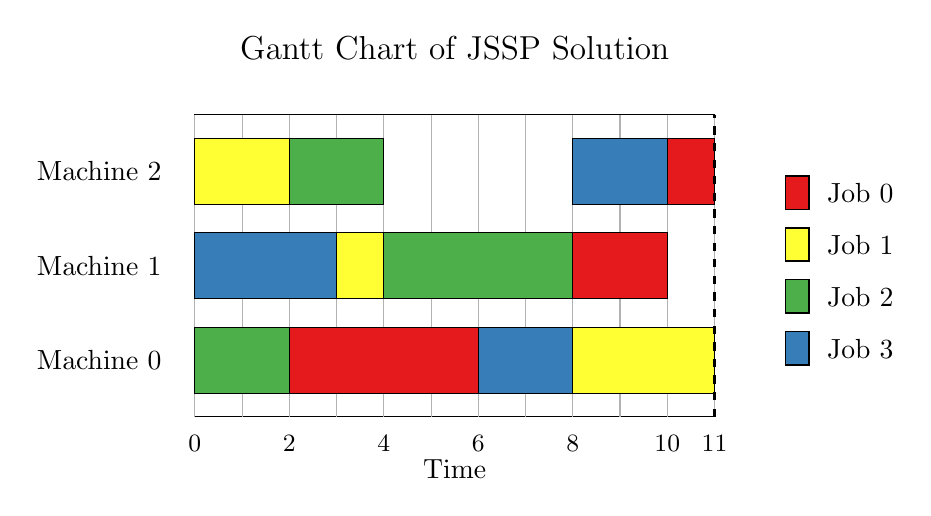
\begin{tikzpicture}[x=0.6cm,y=1.2cm]

% ---- layout parameters ----
\def\Yh{0.35}            % half bar height
\def\yMtwo{2}            % row y for Machine 2
\def\yMone{1}            % row y for Machine 1
\def\yMzero{0}           % row y for Machine 0
\def\xmin{0}
\def\xmax{11}
\def\ymin{-0.6}
\def\ymax{2.6}

% Bar macro (start, end, row y, color)
\newcommand{\gbar}[4]{%
  \fill[#4,draw=black, line width=0.25pt]
    (#1,#3-\Yh) rectangle (#2,#3+\Yh);}

% Plot frame and grid
\draw[black] (\xmin,\ymin) rectangle (\xmax,\ymax);
\foreach \x in {0,...,11}       % integer grid lines
  \draw[gray!60] (\x,\ymin) -- (\x,\ymax);
% label selected ticks
\foreach \x in {0,2,4,6,8,10,11}
  \node[below=3pt] at (\x,\ymin) {\small \x};
% optional half-unit tick at 2.5 (used by a bar)
%\draw[gray!40,densely dashed] (2.5,\ymin) -- (2.5,\ymax);

\node[below=12pt] at ({0.5*(\xmin+\xmax)},\ymin) {Time};
\node[left] at (\xmin-0.5,\yMtwo)  {Machine 2};
\node[left] at (\xmin-0.5,\yMone)  {Machine 1};
\node[left] at (\xmin-0.5,\yMzero) {Machine 0};

% ---- Gantt bars (aligned exactly to the times) ----
% Machine 2
\gbar{0}{2}{\yMtwo}{job1}
\gbar{2}{4}{\yMtwo}{job2}
\gbar{8}{10}{\yMtwo}{job3}
\gbar{10}{11}{\yMtwo}{job0}

% Machine 1
\gbar{0}{3}{\yMone}{job3}
\gbar{3}{4}{\yMone}{job1}
\gbar{4}{8}{\yMone}{job2}
\gbar{8}{10}{\yMone}{job0}

% Machine 0
\gbar{0}{2}{\yMzero}{job2}
\gbar{2}{6}{\yMzero}{job0}
\gbar{6}{8}{\yMzero}{job3}
\gbar{8}{11}{\yMzero}{job1}

% Makespan line at 11
\draw[dashed, thick] (11,\ymin) -- (11,\ymax);

% Legend
\begin{scope}[shift={(12.5,1.6)}]
  \fill[job0,draw=black] (0,0) rectangle +(0.5,0.35); \node[right=3pt] at (0.5,0.175) {Job 0};
  \fill[job1,draw=black] (0,-0.55) rectangle +(0.5,0.35); \node[right=3pt] at (0.5,-0.375) {Job 1};
  \fill[job2,draw=black] (0,-1.10) rectangle +(0.5,0.35); \node[right=3pt] at (0.5,-0.925) {Job 2};
  \fill[job3,draw=black] (0,-1.65) rectangle +(0.5,0.35); \node[right=3pt] at (0.5,-1.475) {Job 3};
\end{scope}

% Title
\node[font=\large] at ({0.5*(\xmin+\xmax)},\ymax+0.7) {Gantt Chart of JSSP Solution};

\end{tikzpicture}
\end{document}
